\documentclass{article}

\usepackage{titlesec}
\usepackage{amsmath}
\usepackage{amsfonts}
\usepackage{graphicx}
\usepackage{float}
\title{Numerical Methods for Ordinary Differential Equations}
\author{Murray Heymann \\
	Technische Universit{\"a}t Kaiserslautern \\
	413121}
\date{\today}


\titleformat{\section}{\normalfont \LARGE \bfseries}
{Problem\ Sheet\ \thesection}{2.3ex plus .2ex}{}
\titleformat{\subsection}{\normalfont \Large \bfseries}
{Question\ \thesubsection}{2.3ex plus .2ex}{}
\titlespacing{\subsubsection}{2em}{*1}{*1}

\begin{document}
\maketitle


\setcounter{section}{2}
\section{}
\subsection{}

\begin{itemize}
	\item[(a)]
		As before, the function $y = e^{- \lambda t}$ was approximated.

		For stepsizes larger than $2/\lambda$, the explicit Euler method
		is not stable.  Indeed this is clearly demonstrated by the
		following graphs, using the implementation from exercise $1$.
		\begin{figure}[H]
			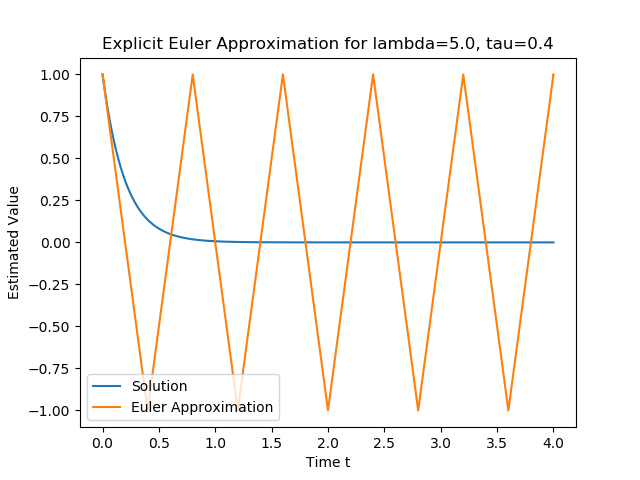
\includegraphics[scale=0.6]{explicit_euler_04}
		\end{figure}
		The approximation certainly does not
		converge to zero, but just jumps between 1 and -1.
		\begin{figure}[H]
			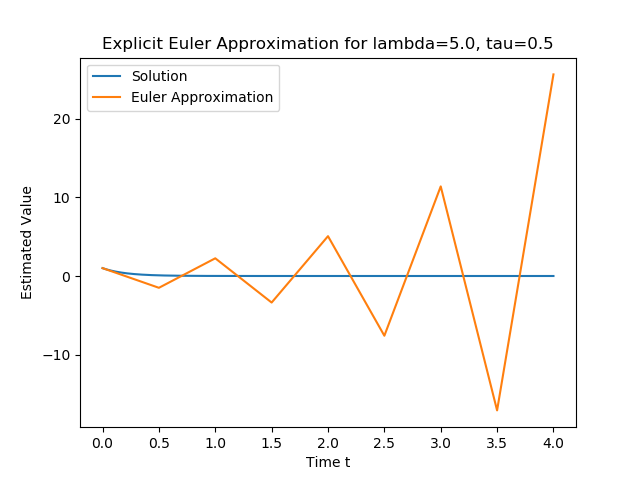
\includegraphics[scale=0.6]{explicit_euler_05}
		\end{figure}
		Here the value has no limit, while the absolute value of the
		approximation goes to infinity.

		Using a much larger $\tau = 0.6$ as stepsize, we see get the
		following approximation using
		the implicit midpoint method:
		\begin{figure}[H]
			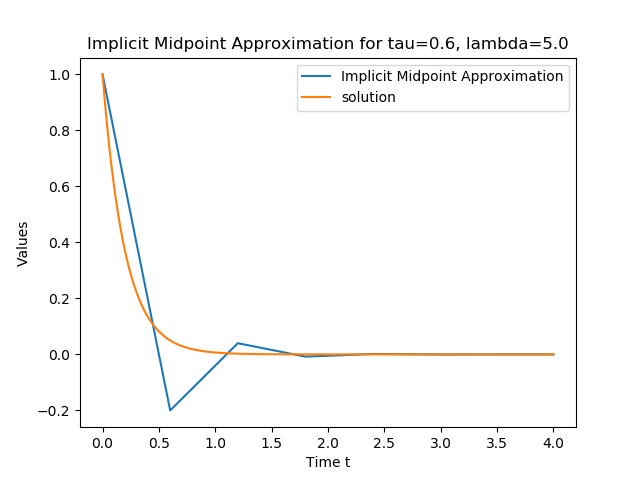
\includegraphics[scale=0.6]{implicit_mid_06}
		\end{figure}
		While it cannot be considered a good approximation in itself, it
		is noticable that the approximation is absolutely convergent to
		$0$, even though our step size is larger than in the explicit
		Euler case. For a stepsize of $\tau=0.2$, which is still
		relatively large, we get the following approximation:
		\begin{figure}[H]
			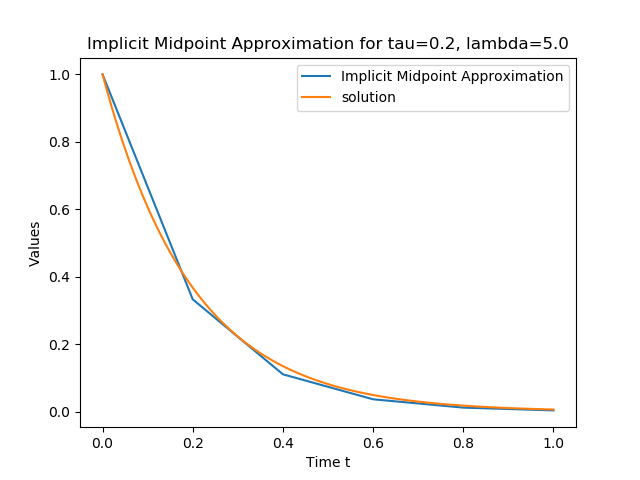
\includegraphics[scale=0.6]{implicit_mid_02}
		\end{figure}
		The local error of the implicit midpoint
		method is shown in the following log-log graph:
		\begin{figure}[H]
			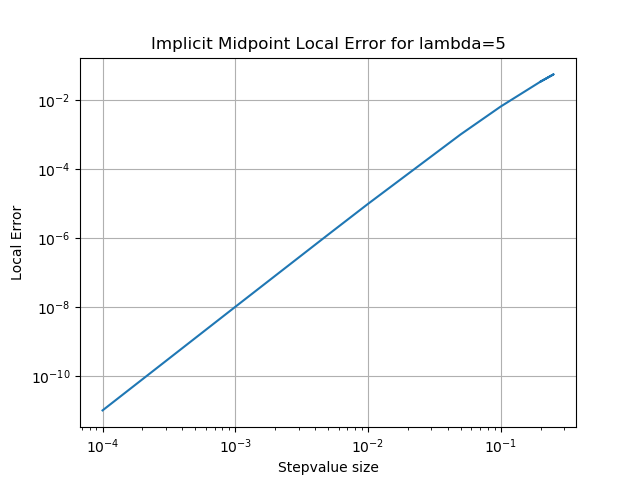
\includegraphics[scale=0.6]{implicit_mid_local_loglog}
		\end{figure}
		The graph is a line with a gradient of about $3$, which is
		consistent with an order $2$ method.
		The global error of the implicit midpoint
		method is shown in the following log-log graph:
		\begin{figure}[H]
			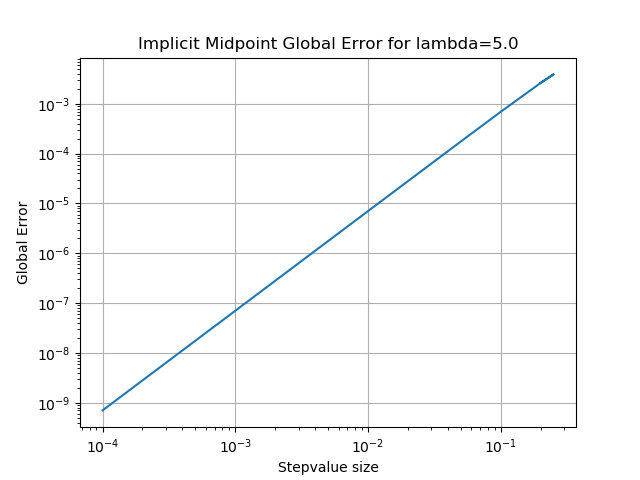
\includegraphics[scale=0.6]{implicit_mid_global_loglog}
		\end{figure}
		It is a line with a gradient of about $2$, which confirms that
		this is an order $2$ method.

		Using $\tau = 0.6$ again as stepsize, we see get the
		following approximation using
		the implicit Gauss method:
		\begin{figure}[H]
			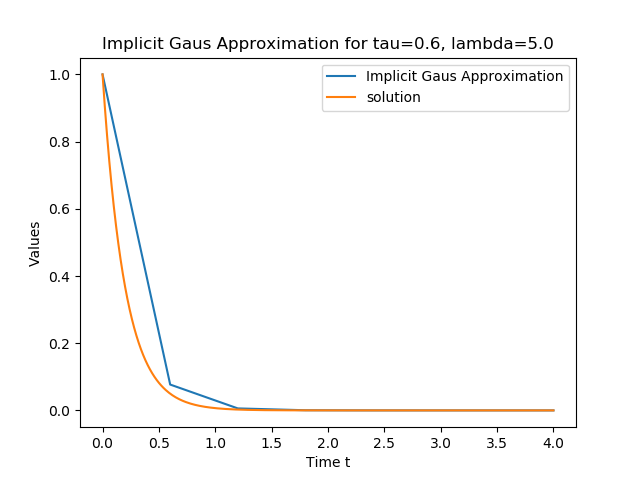
\includegraphics[scale=0.6]{implicit_gauss_06}
		\end{figure}
		It is again
		noticable that the approximation is absolutely convergent to
		$0$, even though our step size is larger than in the explicit
		Euler case. For a stepsize of $\tau=0.2$, which is still
		relatively large, we get the following approximation:
		\begin{figure}[H]
			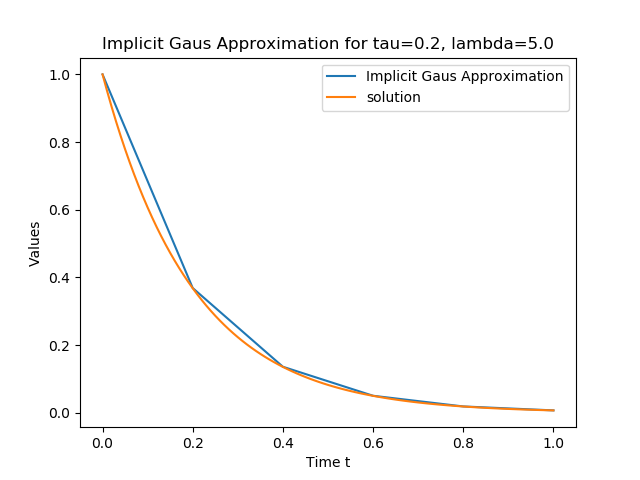
\includegraphics[scale=0.6]{implicit_gauss_02}
		\end{figure}
		The local error of the implicit Gauss
		method is shown in the following log-log graph:
		\begin{figure}[H]
			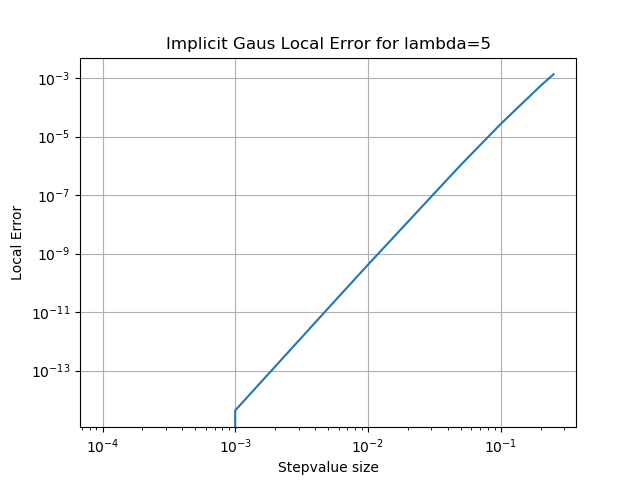
\includegraphics[scale=0.6]{implicit_gauss_local_loglog}
		\end{figure}
		The graph is a line with a gradient of about $5$, which is
		consistent with an order $4$ method.  It should be noted that
		for stepsizes less than $0.001$, the local error was calculated
		as $0$.  This does not mean that there is no error, simply that
		the error was smaller than the implementation can represent as a
		floating point number.
		The global error of the implicit midpoint
		method is shown in the following log-log graph:
		\begin{figure}[H]
			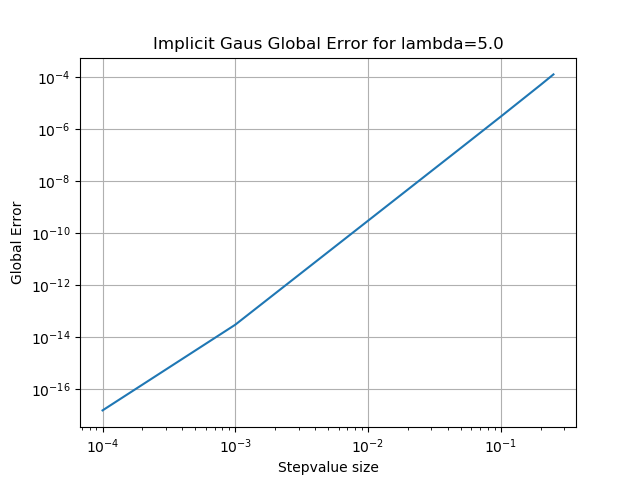
\includegraphics[scale=0.6]{implicit_gauss_global_loglog}
		\end{figure}
		It is a line with a gradient of about $4$, which confirms that
		this is an order $4$ method. For very small stepsizes, the error
		seems to no longer descend along the same curve.  This is most
		likely because of the additional error introduced by Newton's
		method for approximating the $\mathbf{k}_i$'s in the implicit Runge-Kutta
		method. 


\end{itemize}

\begin{figure}[H]
	\includegraphics[scale=0.6]{picture}
\end{figure}

\subsection{}
\begin{itemize}
	\item[(a)]
\end{itemize}
\end{document}
